\documentclass[11pt]{article}

% ---- packages ----
\usepackage[a4paper,margin=2.2cm]{geometry}
\usepackage[T1]{fontenc}
\usepackage{lmodern}
\usepackage{amsmath}
\usepackage{xcolor}
\usepackage{graphicx}
\usepackage{booktabs}
\usepackage{enumitem}
\usepackage{fancyhdr}
\usepackage{titlesec}
\usepackage{textcomp}
\usepackage{tikz}
\usetikzlibrary{arrows.meta,positioning,shapes.geometric,calc}

% ---- brand colours (from echobarrier.com / the Hub UI) ----
\definecolor{ebgreen}{RGB}{2,89,69}
\definecolor{eborange}{RGB}{255,112,38}
\definecolor{ebdark}{RGB}{30,30,30}
\definecolor{ebgrey}{RGB}{107,114,128}
\definecolor{ebline}{RGB}{225,228,226}
\definecolor{ebtint}{RGB}{237,244,242}
\definecolor{eborangetint}{RGB}{255,241,233}

\usepackage{hyperref}
\hypersetup{colorlinks=true,linkcolor=ebgreen,urlcolor=ebgreen}

% ---- headings ----
\titleformat{\section}{\Large\bfseries\color{ebgreen}}{\thesection.}{0.6em}{}
\titleformat{\subsection}{\large\bfseries\color{ebdark}}{\thesubsection}{0.6em}{}
\titlespacing*{\section}{0pt}{1.5em}{0.6em}

% ---- header / footer ----
\pagestyle{fancy}\fancyhf{}
\renewcommand{\headrulewidth}{0.6pt}
\renewcommand{\headrule}{\hbox to\headwidth{\color{ebgreen}\leaders\hrule height \headrulewidth\hfill}}
\lhead{\small\textbf{\color{ebgreen}ECHO BARRIER}\ \small\color{ebgrey}Hub}
\rhead{\small\color{ebgrey}Purchase Order \& Pipeline Guide}
\cfoot{\small\color{ebgrey}\thepage}

% ---- helpers ----
\newcommand{\hubchip}[2]{\tikz[baseline=-0.6ex]\node[fill=#1,text=white,rounded corners=2pt,inner sep=2.5pt,font=\footnotesize\bfseries]{#2};}
\newcommand{\orangebtn}[1]{\hubchip{eborange}{#1}}
\newcommand{\greenbtn}[1]{\hubchip{ebgreen}{#1}}
\newcommand{\greybtn}[1]{\tikz[baseline=-0.6ex]\node[draw=ebgrey,text=ebdark,rounded corners=2pt,inner sep=2.5pt,font=\footnotesize\bfseries]{#1};}
\newcommand{\num}[1]{\tikz[baseline=-0.55ex]\node[circle,fill=eborange,text=white,minimum size=1.5em,inner sep=0pt,font=\small\bfseries]{#1};}
\newcommand{\role}[1]{\textbf{\color{ebgreen}#1}}
\newcommand{\ui}[1]{\textbf{#1}}
\setlist[itemize]{leftmargin=1.4em,itemsep=2.5pt,topsep=3pt}
\setlist[description]{leftmargin=0pt,itemsep=3pt,topsep=3pt,font=\normalfont\bfseries\color{ebdark}}

% callout marker placed in normalised image coords (0,0)=bottom-left .. (1,1)=top-right
\newcommand{\callout}[3]{\node[circle,fill=eborange,text=white,minimum size=1.7em,inner sep=0pt,%
  font=\small\bfseries,draw=white,line width=1.2pt] at (#1,#2) {#3};}
\newcommand{\annotshot}[3]{% #1 image  #2 width(frac of linewidth)  #3 callout body
  \begin{center}\begin{tikzpicture}
  \node[anchor=south west,inner sep=0] (img)
     {\setlength{\fboxsep}{0pt}\setlength{\fboxrule}{0.6pt}\fcolorbox{ebline}{white}{\includegraphics[width=#2\linewidth]{#1}}};
  \begin{scope}[x={($(img.south east)-(img.south west)$)},y={($(img.north west)-(img.south west)$)}]
    #3
  \end{scope}\end{tikzpicture}\end{center}}
\newcommand{\screenshot}[2]{\begin{center}\setlength{\fboxsep}{0pt}\setlength{\fboxrule}{0.6pt}%
  \fcolorbox{ebline}{white}{\includegraphics[width=#2\linewidth]{#1}}\end{center}}
% coloured callout boxes
\newcommand{\whybox}[1]{\par\vspace{3pt}\noindent\colorbox{ebtint}{\parbox{\dimexpr\linewidth-2\fboxsep}%
  {\vspace{3pt}\hspace{2pt}\textbf{\color{ebgreen}Why?} #1\hspace{2pt}\vspace{3pt}}}\par\vspace{3pt}}
\newcommand{\tipbox}[1]{\par\vspace{3pt}\noindent\colorbox{eborangetint}{\parbox{\dimexpr\linewidth-2\fboxsep}%
  {\vspace{3pt}\hspace{2pt}\textbf{\color{eborange}Tip.} #1\hspace{2pt}\vspace{3pt}}}\par\vspace{3pt}}
\newcommand{\legenditem}[2]{\num{#1}~\,#2\quad}

\begin{document}

% =====================================================================
\begin{titlepage}
\thispagestyle{empty}
\vspace*{1.1cm}
\noindent{\color{ebgreen}\rule{\linewidth}{2pt}}\\[0.4cm]
{\noindent\Huge\bfseries\color{ebdark} Echo Barrier Hub}\\[0.25cm]
{\noindent\LARGE\color{ebgreen} Raising Purchase Orders \& the Intercompany Pipeline}\\[0.3cm]
{\noindent\large\color{ebgrey} A hands-on, click-by-click guide for testers}\\[0.2cm]
\noindent{\color{ebgreen}\rule{\linewidth}{2pt}}

\vspace{1.0cm}
\noindent\colorbox{ebtint}{\parbox{\dimexpr\linewidth-2\fboxsep}{\vspace{4pt}
\hspace{4pt}\textbf{\color{ebgreen}What the Hub is.} One internal platform for Echo
Barrier's entire purchase-order journey --- a depot raises an order, it is approved
up the intercompany chain (Depot~$\rightarrow$~EB~Group~$\rightarrow$~EB~SRO), the
supplier manufactures it, and the goods ship back to the depot. Everything ---
approvals, documents, tracking, invoices --- lives in one place, with each person
seeing only what their role needs.\vspace{4pt}}}

\vspace{0.5cm}
\noindent\colorbox{eborangetint}{\parbox{\dimexpr\linewidth-2\fboxsep}{\vspace{4pt}
\hspace{4pt}\textbf{\color{eborange}Please read first --- this is a sandbox.} You are
testing a \emph{staging} copy. It is deliberately \textbf{not} wired to the live
accounting system, so \textbf{judge the workflow and the experience, not the exact
numbers or addresses} (some are still placeholders). Nothing you click here can
affect production or send anything to a supplier.\vspace{4pt}}}

\vspace{0.8cm}
\noindent\textbf{\color{ebgreen}How to read this guide.} Numbered orange markers
(\num{1}, \num{2}, \dots) on each screenshot match the numbered steps in the text ---
they show you \emph{exactly where to click}. Green boxes explain \textbf{why}
something works the way it does.

\vspace{0.6cm}
\noindent\textbf{\color{ebgreen}Where.} \url{https://echo-hub-staging.netlify.app/}
--- your test logins are in \S3.

\vfill
\noindent{\small\color{ebgrey} Echo Barrier Hub --- internal test document.
\textbf{Contains test credentials} --- please don't circulate outside the test group.}
\end{titlepage}

\tableofcontents
\thispagestyle{fancy}

% =====================================================================
\section{Why the Hub works this way}
Before the clicks, the one idea that makes everything else make sense: \textbf{a
depot never buys straight from the factory.} An order is passed \emph{between three
separate Echo Barrier companies}, and each one places its own purchase order with
the next:

\begin{description}
  \item[The depot] (e.g. US~--~Baltimore) needs stock. It raises a request \emph{to
    EB Group}.
  \item[EB Group] (the UK/Ireland company) buys from \emph{EB SRO}.
  \item[EB SRO] (the Slovakian company) places the real manufacturing order with the
    \emph{supplier} (Bamida).
\end{description}

\whybox{Each hop is a genuine sale between two \emph{legal companies}, in different
countries and currencies. That is why every leg is its own purchase order, with its
own approval, its own PO number and its own currency --- it is what customs,
inter\-company transfer pricing, and each company's own accounts require. The Hub
simply makes that chain fast, visible and traceable instead of a pile of emails.}

% =====================================================================
\section{The pipeline at a glance}
Every order travels the same path. Three approval gates move it down the chain; the
cost is shown in each company's own currency, converted automatically.

\vspace{0.3cm}
\begin{center}
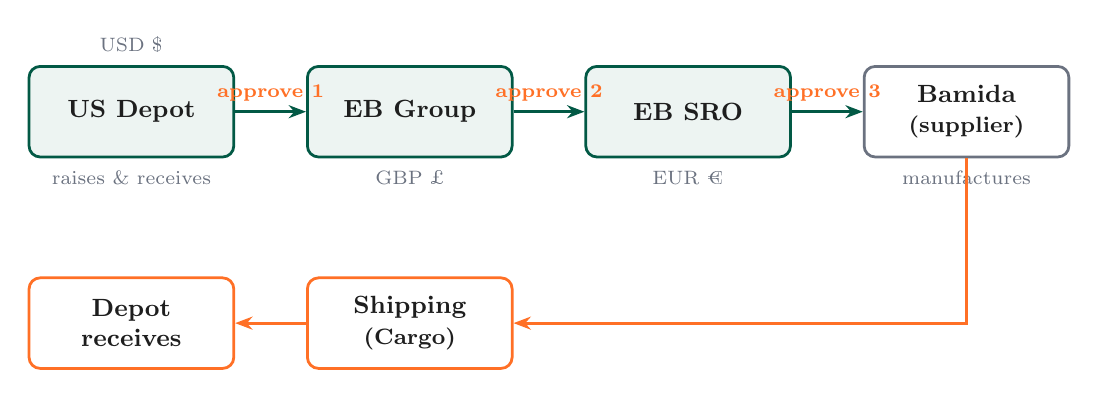
\begin{tikzpicture}[
  node distance=0.55cm and 0.9cm,
  entity/.style={draw=ebgreen,line width=1pt,rounded corners=4pt,fill=ebtint,
     minimum width=2.6cm,minimum height=1.15cm,align=center,font=\small\bfseries,text=ebdark},
  supp/.style={entity,fill=white,draw=ebgrey},
  gate/.style={font=\scriptsize\bfseries,text=eborange,align=center},
  flow/.style={-{Stealth[length=2.2mm]},line width=1pt,color=ebgreen},
  ccy/.style={font=\scriptsize,text=ebgrey}
]
\node[entity] (depot) {US Depot};
\node[entity,right=of depot] (group) {EB Group};
\node[entity,right=of group] (sro) {EB SRO};
\node[supp,right=of sro] (bam) {Bamida\\ \footnotesize(supplier)};
\draw[flow] (depot) -- node[gate,above]{approve 1} (group);
\draw[flow] (group) -- node[gate,above]{approve 2} (sro);
\draw[flow] (sro) -- node[gate,above]{approve 3} (bam);
\node[ccy,below=1pt of depot]{raises \& receives};
\node[ccy,below=1pt of group]{GBP \pounds};
\node[ccy,below=1pt of sro]{EUR \texteuro};
\node[ccy,below=1pt of bam]{manufactures};
\node[ccy,above=1pt of depot]{USD \$};
\node[entity,below=1.5cm of group,fill=white,draw=eborange] (ship) {Shipping\\ \footnotesize(Cargo)};
\node[entity,below=1.5cm of depot,fill=white,draw=eborange] (recv) {Depot\\ receives};
\draw[flow,color=eborange] (bam.south) |- (ship.east);
\draw[flow,color=eborange] (ship) -- (recv);
\end{tikzpicture}
\end{center}

\vspace{0.1cm}
\noindent\begin{tabular}{@{}p{0.30\linewidth}p{0.64\linewidth}@{}}
\toprule
\textbf{\color{ebgreen}Stage} & \textbf{\color{ebgreen}What happens \& who does it} \\
\midrule
Raise & A depot (\role{Sales}) creates the order and sends it for approval. \\
Approve 1 (Depot~$\rightarrow$~Group) & \role{Manager} approves; the Group~$\rightarrow$~SRO order is auto-created. \\
Approve 2 (Group~$\rightarrow$~SRO) & \role{Manager} approves; the SRO~$\rightarrow$~Supplier order is auto-created. \\
Approve 3 (SRO~$\rightarrow$~Supplier) & \role{Manager} approves; the manufacturing order (Bamida) is authorised in accounting. \\
Manufacture, ship, receive & Goods are produced, shipped via Cargo, and received at the depot (\role{Production}). \\
\bottomrule
\end{tabular}

% =====================================================================
\section{Getting in \& finding your way around}
Open \url{https://echo-hub-staging.netlify.app/} and sign in. Three test accounts
are set up for you --- each is a different \emph{role}, so it's worth trying all of
them to see how the Hub changes per person:

\vspace{0.2cm}
\begin{center}
\begin{tabular}{@{}lll@{}}
\toprule
\textbf{\color{ebgreen}Role} & \textbf{\color{ebgreen}Email} & \textbf{\color{ebgreen}Password} \\
\midrule
\role{Manager}    & \texttt{manager@echobarrier.com}    & \texttt{manager-development-2231} \\
\role{Sales}      & \texttt{sales@echobarrier.com}      & \texttt{sales-development-3231} \\
\role{Production} & \texttt{production@echobarrier.com} & \texttt{production-development-4231} \\
\bottomrule
\end{tabular}
\end{center}
\vspace{0.1cm}

\screenshot{img/01-login.png}{0.62}

\noindent Once in, the \textbf{left sidebar} is how you move around. You will only
see the items your role allows:
\begin{description}
  \item[Dashboard] your landing page --- a quick overview.
  \item[Quotes] customer quotations (Sales).
  \item[Purchase Orders] the heart of this guide --- raise, approve and track POs.
  \item[Bill of Materials] the parts \& specs that make up each product.
  \item[Transport] container \& shipment tracking.
  \item[Invoices] intercompany commercial invoices.
  \item[MRP] stock \& manufacturing forecasting.
\end{description}
Your name and a \textbf{Sign~Out} button sit at the bottom of the sidebar.

\whybox{The menu is filtered to your role, so nobody is faced with buttons they
can't use. A \role{Production} user, for instance, never sees prices or the Quotes
page --- only what they need to receive goods.}

% =====================================================================
\section{Raising a purchase order}
This starts the whole pipeline. Do it as a \role{Sales} (or admin) account. In the
sidebar click \ui{Purchase Orders}, then the orange \orangebtn{+ Raise PO} button in
the top-right. You'll see this form:

\annotshot{img/03-raise-po.png}{0.96}{
  \callout{0.315}{0.605}{1}
  \callout{0.71}{0.605}{2}
  \callout{0.33}{0.49}{3}
  \callout{0.345}{0.29}{4}
  \callout{0.625}{0.29}{5}
  \callout{0.80}{0.29}{6}
  \callout{0.845}{0.365}{7}
  \callout{0.815}{0.155}{8}
}

\begin{description}
  \item[\num{1} Raising depot] Choose the depot the stock is for (e.g.
    \texttt{US-BAL}). The small note beneath confirms it is \emph{Raised to
    EB-GROUP} --- every depot order goes to EB Group first.
  \item[\num{2} Delivery address] \textbf{Required} --- where the goods should ship to.
  \item[\num{3} Notes] Anything EB Group should know (priority, context). Free text.
  \item[\num{4} Product] Pick the item. Only real catalogue products appear.
  \item[\num{5} Quantity] How many. A yellow \emph{``Stock short''} hint may appear ---
    it is only a heads-up and never blocks you.
  \item[\num{6} Unit price] The cost (only visible to accounts with cost access). A
    greyed \emph{Xero code} appears under the line so accounting can match it.
  \item[\num{7} Add line] Add more products to the \emph{same} order.
  \item[\num{8} Raise PO for approval] Submits it. The order now sits in the approval
    queue --- you'll see a green ``Purchase order raised'' confirmation.
\end{description}

\tipbox{Order the same things regularly? Fill the form once, then click
\ui{Save as template} (top of the form). Next time, choose it under \ui{Load from
template} and every field is pre-filled.}

\whybox{Notice the PO number is \emph{not} shown yet. The Hub never invents numbers
--- the official one comes from accounting after approval (see \S8). Until then the
order is tracked internally and simply reads ``Awaiting Xero PO number''.}

% =====================================================================
\section{The approval system --- how the chain actually works}
This is the core of the Hub. Approvals are done by a \role{Manager} (or admin).
Click \ui{Purchase Orders} then the \greybtn{Approvals} button (top-right, it shows
an orange count when orders are waiting). Orders are grouped into the three tiers.

\annotshot{img/06-approvals.png}{0.96}{
  \callout{0.315}{0.70}{1}
  \callout{0.37}{0.615}{2}
  \callout{0.765}{0.635}{3}
  \callout{0.835}{0.635}{4}
}

\begin{description}
  \item[\num{1} The tier] Orders are grouped \ui{Approval 1 -- Depot}, \ui{2 --
    Group}, \ui{3 -- SRO}. That number tells you where in the chain the order is.
  \item[\num{2} The order] Each card shows the route
    (\texttt{FROM~$\rightarrow$~TO}, e.g. \texttt{EB-SRO~$\rightarrow$~SUPPLIER}), who
    raised it and when, its line items, and --- when present --- a \emph{ref:} line
    linking it back to the order it came from, so the chain is traceable right back
    to the depot that started it.
  \item[\num{3} Reject] Stops the chain at this tier (you can add a reason).
  \item[\num{4} Approve] Advances the order --- see below.
\end{description}

\subsection{What ``Approve'' actually does}
Approving a tier does three things \emph{in one atomic step} (all-or-nothing):
\begin{enumerate}[leftmargin=1.8em,itemsep=3pt]
  \item marks this leg \textbf{approved}, recording \emph{who} approved it and
    \emph{when};
  \item automatically \textbf{raises the next leg} into the queue --- so approving the
    Depot order makes the Group order appear, approving Group makes the SRO order
    appear, and so on --- carrying the \textbf{reference} forward;
  \item hands the approved leg to \textbf{accounting}, which creates the real
    purchase order and sends its official \textbf{Xero PO number} back to the Hub.
\end{enumerate}
So you approve three times in total, and the order walks itself down the chain:
\[
\text{Depot}\ \xrightarrow{\text{approve 1}}\ \text{Group}\ \xrightarrow{\text{approve 2}}\ \text{SRO}\ \xrightarrow{\text{approve 3}}\ \text{Supplier (Bamida)}
\]

\whybox{We made approval a single atomic step (rather than ``mark approved'', then
separately ``create the next order'') so a half-finished approval can never leave an
order stranded with no next step --- an earlier problem this design fixed. It also
means two managers clicking at once can't accidentally create a duplicate order.}

\tipbox{\ui{Approval~3 -- SRO} is the one that authorises real manufacturing. In this
sandbox that hand-off is switched off, so nothing reaches a supplier --- approve it
freely to see the flow complete.}

% =====================================================================
\section{Tracking every order on the board}
Clicking \ui{Purchase Orders} opens the \textbf{board}. This is your live map of
every order.

\annotshot{img/04-board.png}{0.99}{
  \callout{0.87}{0.885}{1}
  \callout{0.945}{0.885}{2}
  \callout{0.50}{0.77}{3}
  \callout{0.235}{0.685}{4}
  \callout{0.795}{0.685}{5}
  \callout{0.285}{0.63}{6}
  \callout{0.26}{0.455}{7}
}

\begin{description}
  \item[\num{1} Approvals] Jump to the approval queue (\S6); the badge shows how many
    are waiting.
  \item[\num{2} + Raise PO] Start a new order (\S5).
  \item[\num{3} Status tiles] At-a-glance counts --- Total Active, Awaiting Approval,
    In Manufacturing, Shipping.
  \item[\num{4} Kanban / Table] Switch between the card board and a dense table.
  \item[\num{5} Search] Filter by PO number, entity, status or SKU.
  \item[\num{6} Lifecycle columns] The order's journey, left to right:
    \emph{Depot~$\rightarrow$~Group}, \emph{Group~$\rightarrow$~S.R.O}, \emph{S.R.O},
    \emph{Sent to manufacturing}, \emph{Manufacturing in progress}, \emph{Shipping}.
    A \role{Manager} can \textbf{drag a card} to the next stage. \emph{(The exact
    manufacturing stage names are provisional --- feedback welcome.)}
  \item[\num{7} PO number] A real Xero number (e.g. \texttt{EBUSA26013}) once
    approved; otherwise the card reads \textbf{``Awaiting Xero PO number''}. Each card
    also shows its route, SKU count and age.
\end{description}

\whybox{``Awaiting Xero PO number'' is deliberate. The Hub isn't the book of record
for PO numbers --- accounting is. Rather than invent a number the Hub would later
have to reconcile, a card honestly shows it's waiting, then updates the moment the
official number arrives. So you always see the \emph{real} number or a clear
``not yet''.}

\subsection{How to read the PO numbers}
The numbers follow \textbf{our own entity-prefixed scheme}, so one glance tells you
whose order it is and which leg of the chain you're looking at:

\vspace{0.15cm}
\begin{center}
\begin{tabular}{@{}llp{0.46\linewidth}@{}}
\toprule
\textbf{\color{ebgreen}Example} & \textbf{\color{ebgreen}Leg} & \textbf{\color{ebgreen}Meaning} \\
\midrule
\texttt{EBUSA26013}       & Depot $\rightarrow$ Group     & The US depot's order to EB Group (USD). \\
\texttt{EBG26086}         & Group $\rightarrow$ SRO       & EB Group's order to EB SRO (GBP), referencing the depot PO. \\
\texttt{EBSRO26013-01}    & SRO $\rightarrow$ Supplier    & EB SRO's order (EUR). The suffix is the document's \emph{purpose}: \texttt{-01} manufacturing spec, \texttt{-02} shipping/cargo, \texttt{-03} accounting. \\
\bottomrule
\end{tabular}
\end{center}
\vspace{0.1cm}

\noindent Each leg's \emph{Reference} points at the number one step up the chain, so
the whole journey is traceable from the supplier order right back to the depot
request. The full numbering scheme --- with a worked example of all five documents
--- is in the companion document \textbf{\texttt{po-flow.pdf}}.

% =====================================================================
\section{The purchase-order document --- and where to download the PDF}
\textbf{Click any card} on the board to open its \textbf{detail panel} on the right.
The green \greenbtn{Download PDF} button sits right at the \emph{top} of that panel.

\annotshot{img/05-po-panel.png}{0.96}{
  \callout{0.865}{0.89}{1}
  \callout{0.755}{0.805}{2}
  \callout{0.755}{0.70}{3}
  \callout{0.755}{0.485}{4}
}

\begin{description}
  \item[\num{1} Download PDF] The green button, right at the top --- generates the
    branded purchase order (see below).
  \item[\num{2} Status] Where the order is (Requested, Approved, \dots).
  \item[\num{3} Route] The from~$\rightarrow$~to entities for this leg.
  \item[\num{4} Timeline, shipment \& attachments] Created/approved dates, the linked
    Cargo shipment, and any files. Orders that carry line items also show a
    \emph{Line items \& deliveries} section here, with received quantities.
\end{description}

\noindent The downloaded PDF is the real, branded document: Echo Barrier logo, the
\textbf{PO Number} then the \textbf{Reference} beneath it, both companies' full
\textbf{addresses} (From / To), \textbf{who approved it}, the line items, and the
\textbf{total in that leg's currency}.

\whybox{The total is shown in each leg's own currency --- the US depot order in USD,
the EB~Group order in GBP, the EB~SRO order in EUR --- even though the cost is only
entered once. The Hub converts it automatically at the current weekly rate, because
each company's paperwork and accounts must be in \emph{its} currency. Prices are
hidden entirely from accounts without cost access (e.g. \role{Production}), so the
same PO can safely go to the factory floor as a spec-only document.}

% =====================================================================
\section{Commercial invoices}
When a container ships, a \role{Manager} raises the intercompany \textbf{commercial
invoice} from the \ui{Invoices} page.

\annotshot{img/07-invoices.png}{0.96}{
  \callout{0.29}{0.795}{1}
  \callout{0.92}{0.635}{2}
  \callout{0.26}{0.315}{3}
}

\begin{description}
  \item[\num{1} New invoice from a container] Pick the container the goods shipped in.
  \item[\num{2} EUR / USD leg] Choose the leg: EUR for SRO~$\rightarrow$~Group, USD for
    Group~$\rightarrow$~USA. The Hub builds the document with values, FX and lines.
  \item[\num{3} Issued invoices] Every invoice raised is listed here to review,
    download or void.
\end{description}

\whybox{Invoice creation lives on the \emph{Invoices} page (not Transport) because
that is where someone doing invoicing naturally looks --- create and manage in one
place.}

% =====================================================================
\section{Your role, and why prices are sometimes hidden}
\begin{center}
\begin{tabular}{@{}lp{0.60\linewidth}@{}}
\toprule
\textbf{\color{ebgreen}Role} & \textbf{\color{ebgreen}Can do} \\
\midrule
\role{Manager}    & View \& \textbf{approve} POs; receive deliveries; view BOM \& \textbf{costs}; create \& view commercial invoices; MRP forecasting; transport. \\
\role{Sales}      & Create \& send quotes; \textbf{raise} POs; view POs. \\
\role{Production} & View \& \textbf{receive} POs; view the BOM (\emph{specs only, no prices}); transport. \\
\bottomrule
\end{tabular}
\end{center}

\whybox{Cost visibility is a separate permission. Warehouse and production staff can
see everything they need to receive and build --- SKUs, quantities, specs --- but not
prices. That way the very same purchase order can be handed to the factory floor
without exposing commercial pricing.}

\vspace{0.4cm}
\noindent{\color{ebgreen}\rule{\linewidth}{1pt}}\\[0.2cm]
\noindent{\small\color{ebgrey} Found something confusing, broken or missing? That is
exactly what this test is for. Please note \emph{which account}, \emph{which screen}
and \emph{what you expected}, and send it back. Thank you for helping shape the Hub.}

\end{document}
